
\chapter{Introduction} 
\label{sec:introduction}
	
	This machine learning master thesis is about neural-networks (section \ref{sec:neural_networks}). We'll investigate on a technique called adversarial-learning (section \ref{sec:adversarial_learning}) to know if it can help neural-networks in performing better.


	\section{Motivation}
		At the very beginning of this thesis, there is me, the writer. I wanted, from the very first day, to work on neural-networks and more specifically on deep-learning. I wanted so, because neural-networks has become in the last decade the most efficient algorithm at classifying images. 
		I was then searching for a topic. I discovered the work made by Ian J. Goodfellow, Jonathon Shlens and Christian Szegedy. In their publication named "Explaining and Harnessing Adversarial Examples"\cite{goodfellow2014explaining} they motivate that adversarial learning could improve the accuracy of some given neural-networks. After contacting one of the authors of this publication, it appeared that it would be a good contribution to validate their observations on other datasets, since most of their test are based on the MNIST dataset\cite{lecunmnist}. Therefore, the following thesis is about further understanding and validating the proposed adversarial-learning method described in \cite{goodfellow2014explaining} with different parameter and different databases.

	\section{Methodology}
		We are therefore going to investigate on how is adversarial-learning performing on specific neural-networks called shallow-neural-networks. For the investigation we'll evaluate the impact of different parameters on the model, we are going to compare the adversarial-model with some others and will also evaluate few adversarial-models on different databases. On the same time, we are going to investigate on the reasons underlining the adversarial performances. To do so, we will first re-implement the proposed solution of \cite{goodfellow2014explaining} in such a way that we isolate adversarial-learning from other techniques used in the paper. At this point we will emphasize the benefits of adversarial-learning.

		We will then move to another dataset similar to the first one, there will also be 10 different classes of images to classify. That dataset will be the CIFAR10\cite{krizhevsky2009learning}. Again, some knowledge will be acquired from this experience. Finally, we will test the adversarial-learning on a dataset of other nature. The one we will try is a tree location dataset: the Covertype dataset\footnote{\url{https://archive.ics.uci.edu/ml/datasets/Covertype}}. The results obtained from this dataset bring new insights on adversarial-learning.

	\section{Expected outcome}
		In their paper, Ian J. Goodfellow, Jonathon Shlens and Christian Szegedy, described classic shallow-neural-networks to be too linear in what they learn. by linear they meant that the classifier was too much feating the data distribution given on the train-set. With adversarial-learning, they aim at learning a classifier relying less on the inputs data as such but better relying on the idea of the class.
		
		At the end of the report, one can expect to better understand adversarial learning. One can expect understanding the advantages of adversarial-learning on a more classic approach to learning. Also, we'll demonstrate that this learning technique generalizes to other datasets.

	\section{Adversarial-learning}
		Until now, we've been speaking a lot of adversarial-learning without explaining what it is about. Lets start off with mentioning what an adversarial sample to a classifier would be. Imagine you have full knowledge of a given classifier. Starting from there, you can create samples to this classifier that are going to give some predictions. Knowing how does the classifier behaves, you can creates samples leading your classifier to some mistakes. This are adversarial samples. In machine learning, adversarial-learning is about creating a classifier resisting to adversarial samples.

		In the publication that interest us\cite{goodfellow2014explaining}, the authors noticed that twisting each pixels of the input images by some very specific values (the adversarial values), an accurate classifier could be easily fooled. Lets detail : Consider you have a classifier able to recognize the MNIST dataset and this classifier makes 10 errors when guessing the classes of 200 samples ($95\%$ accuracy). Now, if you modify each pixels of these 200 samples by a little value, the classifier makes 180 errors ($10\%$ accuracy). You've fooled your classifier with adversarial samples.

		The adversarial-learning algorithm we use is going to learn from adversarial samples. Therefore, at any time the algorithm want to predict the class of a sample, he will predict the class of the adversarial sample. It's with this approach that we aim at augmenting the accuracy of the classifier.


	\section{Running example, the 'simple example'}
		On the next sections we will explain what are neural-networks, how do we train them and how adversarial-learning apply to them. All along these explanations we will use an example called the "simple example" to illustrate our definitions.


		The \textbf{task} of our example is to predict the class of an image. There is 3 types of images, a \textit{dot}, a \textit{column} and a \textit{comma}. When a sample is called to be a \textit{dot}, it is referred as belonging to class $y=1$. When it's a \textit{comma}, a class $y=2$ and a \textit{column} a class $y=3$.

		The \textbf{inputs} to our examples are images. They are gray-scaled and have 3 pixels with values in range $[0,1]$. The 3 pixels are aligned in a column such that there is an upper pixel ($x_1$), a middle pixel ($x_2$) and a lower pixel ($x_3$). 

		On the training dataset we have 2 samples for each classes. It is with these examples that we are going to train our classifier.
		$$ \boldsymbol{x}^1 = \left( \begin{matrix} 0  \\ 0  \\ 1  \end{matrix}\right) \text{ ; }
		   \boldsymbol{x}^2 = \left( \begin{matrix} 0  \\ .1 \\ .9 \end{matrix}\right) \text{ ; }
		   y^1 = y^2 = 1 $$

		$$ \boldsymbol{x}^3 = \left( \begin{matrix} 0  \\ 1  \\ 1  \end{matrix}\right) \text{ ; }
		   \boldsymbol{x}^4 = \left( \begin{matrix} .1 \\ .9 \\ .9 \end{matrix}\right) \text{ ; }
		   y^3 = y^4 = 2 $$

		$$ \boldsymbol{x}^5 = \left( \begin{matrix} 1  \\ 0  \\ 1  \end{matrix}\right) \text{ ; }
		   \boldsymbol{x}^6 = \left( \begin{matrix} .9 \\ .1 \\ .9 \end{matrix}\right) \text{ ; }
		   y^5 = y^6 = 3 $$
		Where $\boldsymbol{x}^i$ refer to the input sample $i$ and $y^i$ refer to the class of sample $i$.

		The \textbf{model} we are going to use is a neural-network. Because it has few layers, it's also referred as a shallow-neural-network. Our simple neural-network will have 3 inputs, one for each pixel of the images, 3 hidden neurons and 3 output neurons. \Fref{fig:simple_NN} is a graphical representation of our model.

		\vskip 1cm
		\textbf{Notation: }\\
		$y$ is the class of a sample. This $y$ is an integer representation of the class (1, 2, 3 ...). We'll often use the 'one-hot' notation of this value. For instance, if there is 3 possible classes, the one-hot version of $y=2$ will be $\boldsymbol{y} = [0,1,0]$. Where the second value of $\boldsymbol{y}$ is '1' and all the rest are '0'.

		\begin{figure}
			\centering
			\def\layersep{2cm}	
			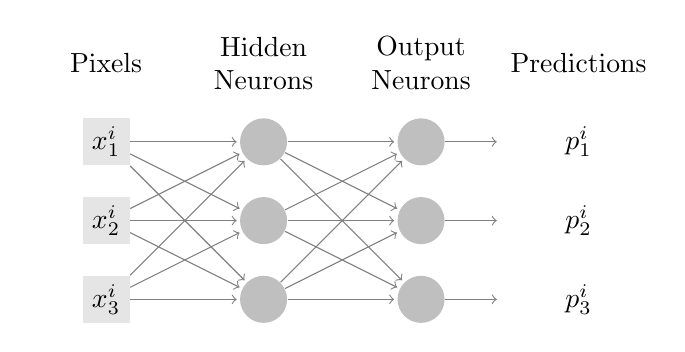
\begin{tikzpicture}[shorten >=1pt,->,draw=black!50, node distance=\layersep]
			    \tikzstyle{every pin edge}=[<-,shorten <=1pt]
			    \tikzstyle{pixel} = [rectangle, fill=black!10,minimum size=17pt,inner sep=0pt]
			    \tikzstyle{neuron}=[circle,fill=black!25,minimum size=17pt,inner sep=0pt]
			    \tikzstyle{annot} = [text width=5em, text centered]
			    \tikzstyle{annot2} = [text width=18em, text centered]
				\tikzstyle{accolade} = [rectangle, text centered, minimum size=17pt]
			    
			    %%% DRAW THE NODES
			    \foreach \name / \y in {1,2,3}
			        \node[pixel] (I-\name) at (0,-\y) {$x^i_\y$};
			    \foreach \name / \y in {1,...,3}
					\node[neuron] (H-\y) at (\layersep*1,-\y) {};
				\foreach \name / \y in {1,...,3}	
					\node[neuron] (O-\y) at (\layersep*2,-\y) {};
				\foreach \name / \y in {1,...,3}
					\node[annot] (P-\y) at (\layersep*3,-\y) {$p^i_\y$};

			    %%% DRAW THE PATHS
			    \foreach \source in {1,...,3}
			        \foreach \dest in {1,...,3}
			            \path (I-\source) edge (H-\dest);

			    \foreach \source in {1,...,3}
			        \foreach \dest in {1,...,3}
			            \path (H-\source) edge (O-\dest);

			    \foreach \source in {1,...,3}
			            \path (O-\source) edge (P-\source);

			    %%% ANOTATE
			    \node[annot,above of=I-1, node distance=1cm] (iv) {Pixels};
			    \node[annot,above of=H-1, node distance=1cm] () {Hidden Neurons};
			    \node[annot,above of=O-1, node distance=1cm] () {Output Neurons};
			    \node[annot,above of=P-1, node distance=1cm] () {Predictions};

			\end{tikzpicture}
			\caption{Simple example of shallow-neural-network}
			\label{fig:simple_NN}
		\end{figure}










	% 	To understand our adversarial training we will use a simple neural network composed by two sigmoid neurons (see section \ref{sec:Artificial_neurons}). The network aims a recognizing a columns and a dot in a three by one pixels image. This network is sketched on \fref{fig:2N_NN}. Considering a white pixel has value $1$ and a dark pixel has value $0$, a column could be represented by a vector $x^1 = [1,0,1]$ and a dot could be by $x^2 = [0,0,1]$. We consider the column to be the output $y^i = 0$ and the dot to be the output $y^i = 1$
	% 	To predict a sensible value, a two-sigmoid network could use the weights and biases :
	% 	$$ W = \left( \begin{matrix} 1 & -1 \\ -1 & -1 \\ 1 & 1 \end{matrix} \right) ; b = \left( \begin{matrix} -1.5 & 0.5 \end{matrix} \right)$$
		
	% 	\vskip 1em
	% 	\textbf{signal propagation: } The input signal $x^i$ propagates through the network resulting in a prediction vector $p^i = \sigma(W^Tx + b)$. To know how right or wrong is this prediction vector, we would use a cost function like the negative log-likelihood:
	% 	$$ C^i = y^i \ln(p^i) + (1-y^i)\ln(1-p^i) $$
	% 	Propagating $x^1$ and $x^2$, we get that $p^1 = [\sigma(.5), \sigma(-.5)]$ and $p^2 = [\sigma(-.5), \sigma(.5)]$

	% 	\begin{figure}
	% 		\centering
	% 		\def\layersep{1.5cm}	
	% 		\begin{tikzpicture}[shorten >=1pt,->,draw=black!50, node distance=\layersep]
	% 		    \tikzstyle{every pin edge}=[<-,shorten <=1pt]
	% 		    \tikzstyle{pixel} = [rectangle, fill=black!10,minimum size=17pt,inner sep=0pt]
	% 		    \tikzstyle{neuron}=[circle,fill=black!25,minimum size=17pt,inner sep=0pt]
	% 		    \tikzstyle{annot} = [text width=5em, text centered]
	% 		    \tikzstyle{annot2} = [text width=18em, text centered]
	% 			\tikzstyle{accolade} = [rectangle, text centered, minimum size=17pt]
			    
	% 		    %%% DRAW THE NODES
	% 		    \foreach \name / \y in {1,2,3}
	% 		        \node[pixel] (I-\name) at (0,-\y) {$x^i_\y$};
	% 		    \node[] (I-4) at (\layersep/2,-3.5) {$1$};
	% 		    \foreach \name / \y in {1,2}
	% 				\node[neuron] (O-\y) at (\layersep*2,-\y-0.5) {$\sigma(z_\y)$};
	% 			\foreach \name / \y in {1,2}	
	% 				\node[] (C-\y) at (\layersep*3,-\y-0.5) {$p^i_\y$};

	% 		    %%% DRAW THE PATHS
	% 		    \foreach \source in {1,...,4}
	% 		        \foreach \dest in {1,2}
	% 		            \path (I-\source) edge (O-\dest);
	% 		    \foreach \y in {1,2}
	% 		        \path (O-\y) edge (C-\y);

	% 		    %%% ANOTATE
	% 		    \node[accolade] at (\layersep*3+1em,-2) { \Huge\} };
	% 		    \node[annot2] at (\layersep*3+10.5em,-2) (cost) {$C^i = \sum_k y^i_k \ln(p^i_k) + (1-y^i_k)\ln(1-p^i_k) $};

	% 		    \node[annot,above of=I-1, node distance=1cm] (iv) {Pixels};
	% 		    \node[annot,above of=O-1, node distance=1cm] (iv) {Neurons};
	% 		    \node[annot,above of=cost, node distance=1cm] (iv) {Cost};

	% 		\end{tikzpicture}
	% 		\label{fig:2N_NN}
	% 		\caption{Two neurons neural network}
	% 	\end{figure}


	% \section{Adversarial learning}
	% 	Imagine you are allowed to modify each pixels of our image by a value $\epsilon$. Intuitively, if you want to improve the recognition, you would increase the contrast in the picture and insist on the dots where the aught to be. On the other hand, if you want to confuse the recognition, you would lower the contrast and add color where there shouldn't be.

	% 	These properties are the ones we aught to enforce with our adversarial learning. For an epsilon small enough, we subtract to $x^i$ $\epsilon$ times the sign of the derivative with respect to $x^i$ of the Cost $C^i$.
	% 	$$ x^{i_{\text{adv}}} \leftarrow x^i - \epsilon \text{ sign}(\nabla_{x^i} C^i) $$
	% 	Therefore the input $x^i$ is modified such that ?? TODO: HERE IS THE THING ??

	% 	\vskip 1em
	% 	\textbf{In our example. } We apply the adversarial learning to our example. First we compute the derivative of the Cost with respect to $x^i$. (The mathematics behind this derivative is detailed on the appendix \ref{sec:2N_NN_cost})
	% 	$$	\frac{\delta C^i}{\delta x^i} = W \cdot \left( y^i -p^i \right) $$
	% 	Then we subtract the sign of this derivative to the actual input $x^i$
	% 	\begin{equation}
	% 		\begin{split}
	% 			x^{1_{\text{adv}}} &\leftarrow x^1 - \epsilon \text{ sign}(\nabla_{x^1} C(W,b,x^1)) \\
	% 			x^{1_{\text{adv}}} &\leftarrow x^1 - \epsilon \text{ sign}( W \cdot ( y^i -p^i) )
	% 		\end{split}
	% 	\end{equation}
	% 	\begin{equation}
	% 		x^1 = \left( \begin{matrix} 1 \\ 0 \\ 1 \end{matrix} \right) ;
	% 		x^{1_{\text{adv}}} = \left( \begin{matrix} .7 \\ 0 \\ 1 \end{matrix} \right) ;
	% 		x^2 = \left( \begin{matrix} 0 \\ 0 \\ 1 \end{matrix} \right) ;
	% 		x^{2_{\text{adv}}} = \left( \begin{matrix} .3 \\ 0 \\ 1 \end{matrix} \right) ;
	% 	\end{equation}
		


	% 	Once we have these derivatives, the worst modification we can make to sample $x^i$ is by following this derivative. 
		

	% \section{Dataset}
	% 	The first dataset we will be using is the MNIST\ref{??} dataset. This dataset is composed by 60k gray scale images. Each of them represent a hand written digit (6k of each). 
